\documentclass[useAMS,usenatbib]{mn2e}
\usepackage[toc,page]{appendix}
\usepackage{natbib}
\usepackage{amssymb}
\usepackage{epsf}
\usepackage{pstricks}
\usepackage{color}
\usepackage{graphicx}
\usepackage{slashed}
\usepackage{relsize}
%\usepackage{float}
\usepackage{morefloats}
\usepackage{multirow}

\usepackage{amsmath}
\usepackage{amsxtra}
\usepackage{amsbsy}
\usepackage{amscd}
\usepackage{array}
\usepackage{url}

%\usepackage {graphics}
%\usepackage {amsfonts}
%\usepackage {indentfirst}
%\usepackage{verbatim}

%\usepackage {a4wide}
%\usepackage {setspace}
%\usepackage{enumitem}
\usepackage{hyperref}
%\usepackage[all]{hypcap}
%\usepackage{caption}
\usepackage[justification=centering]{caption}

\newcommand{\nat}{Nature}
\newcommand{\mnras}{MNRAS}
\newcommand{\apj}{ApJ}
\newcommand{\apjl}{ApJL}
\newcommand{\apjs}{ApJS}
\newcommand{\aap}{A\&A}
\newcommand{\pasa}{PASA}
\newcommand{\apss}{ApSS}
\newcommand{\araa}{ARAA}
\newcommand{\aj}{Astron. J.}
\newcommand{\aaps}{A\&AS}

%\topmargin=-0.4in

%%%%%%%%%%%%%%%%%%%%%%%%%%%%%%%%%%%%%%%%%%%%%%%%%%%%%%%%%%%%%%%%%%%%%%
\bibliographystyle{mn2e}

\begin{document}

\title[Wideband High Precision Pulsar Timing]{Wideband High Precision Pulsar Timing}

%\author[S. Dai et al.]{S. Dai$^{1,2}$, G. Hobbs$^2$, R. Shannon$^2$, M. Kerr$^2$, W. A. Coles$^3$, R. N. Manchester$^1$, 
%\newauthor W. van Straten$^4$, M. Bailes$^4$, N. D. R. Bhat$^5$, S. Burke-Spolaor$^6$, M. J. Keith$^7$, 
%\newauthor Y. Levin$^8$,S. Os\l owski$^{9,10}$, D. Reardon$^8$, V. Ravi$^{11}$, J. M. Sarkissian$^{12}$, L. Toomey$^{2}$, 
%\newauthor J.-B. Wang$^{13}$, L. Wen$^{14}$, X.-J. Zhu$^{14}$\\
%$^1$School of Physics and State Key Laboratory of Nuclear Physics and Technology, Peking University, Beijing 100871, China\\
%$^2$CSIRO Astronomy and Space Science, Australia Telescope National Facility, Box 76 Epping NSW 1710, Australia\\
%$^3$Department of Electrical and Computer Engineering, University of California, San Diego, La Jolla, CA 92093, USA\\
%$^4$Centre for Astrophysics and Supercomputing, Swinburne University of Technology, PO Box 218, Hawthorn, VIC 3122, Australia\\
%$^5$International Centre for Radio Astronomy Research, Curtin University, Bentley, WA 6102, Australia\\
%$^6$Department of Astronomy, California Institute of Technology, Pasadena, CA 91125, USA\\
%$^7$Jodrell Bank Centre for Astrophysics, University of Manchester, M13 9PL, UK\\
%$^8$School of Physics, Monash University, PO Box 27 Clayton, VIC 3800, Australia\\
%$^9$Max-Planck-Institut f\"{u}r Radioastronomie, Auf dem H\"{u}gel 69, D-53121 Bonn, Germany\\
%$^{10}$Department of Physics, Universit\"{a}t Bielefeld Universit\"{a}tsstr. 25 D-33615 Bielefeld, Germany\\
%$^{11}$School of Physics, University of Melbourne, Parkville, VIC 3010, Australia\\
%$^{12}$CSIRO Astronomy and Space Science, Parkes Observatory, Box 276, Parkes NSW 2870, Australia\\
%$^{13}$Xinjiang Astronomical Observatory, Chinese Academy of Sciences, 150 Science 1-Street, Urumqi, Xinjiang 830011, China\\
%$^{14}$Department of Physics, University of Western Australia, Crawley, WA 6009, Australia\\
%}

\maketitle

\begin{abstract}

We investigate various frequency-dependent effects on the precision of pulsar timing, especially 
for wideband pulsar timing. This requires accounting for the frequency evolution of the pulse 
profile, dispersive delay and effects such as the interstellar scintillation and Doppler shift 
caused by the motion of the Earth around the Sun. 
%
In order to test our algorithm, we use a new simulation software package that can simulate realistic 
observations in PSRFITS format with frequency evolution of pulse profile, dispersion measure variations 
and interstellar scintillation. 
%
With our simulated data sets, we show that currently available timing techniques, which fully average
pulse profiles in frequency cannot account for above frequency-dependent effects properly, and therefore 
increase the noise level of a given data set.
%

We apply our algorithms to Parkes Pulsar Timing Array (PPTA) data sets, and show how the timing 
precision and dispersion measure determination can be improved compared with existing methods.

We also carry out studies on pulsar timing with future Ultra-wideband receiver system being 
developed at CSIRO Astronomy and Space Science. Through simulations we discuss and investigate the 
effects of dispersion measure variation, profile evolution and scintillation. 
%
We demonstrate the importance of applying new timing algorithms for wideband receiver systems.

\end{abstract}



\begin{keywords}
%
pulsars: general
%
\end{keywords}


\section{Introduction}

The pulsar timing method has numerous applications. It is used to test theories of 
gravity~\citep[e.g.,][]{Kramer06}, to determine pulsar properties~\citep[e.g.,][]{Antoniadis} 
and to study the interstellar medium~\citep[e.g.,][]{Keith13}. In pulsar timing array (PTA) 
projects the pulse times of arrival (ToAs) are compared between different pulsars with the 
aim of identifying correlated signals that are caused by gravitational waves passing the 
Earth or the pulsars~\citep[e.g.,][]{Foster90}. Pulsar timing data sets become more sensitive 
as the ToA precision increases. The most straightforward way to increase this precision 
is to increase the signal-to-noise (S/N) ratio of the pulse profile. This can be done using 
longer observation times, more sensitive receiver systems or by increasing the observation 
bandwidth. 

The pulsar timing method relies on the stability of the averaged pulse profiles. The Parkes 
Pulsar Timing Array (PPTA) project currently uses two receiver systems~\citep{Manchester13}. 
One provides 256\,MHz of bandwidth around $\sim$1400\,MHz. The other simultaneously provides 
64\,MHz around 740\,MHz and 1024\,MHz around 3100\,MHz. For the initial PPTA data release, 
in order to obtain stable, S/N average pulse profiles, we fully average data sets in frequency 
across each observing band. An analytic template was made for each observing band for each pulsar. 
The ToAs were then determined by cross-correlating those templates with the actual data sets.  

This methodology is not perfect. It requires a method to align the analytic templates 
between different observing bands for each pulsar. The pulse profiles must also be unchanging. 
However, this averaging process can lead to apparent pulse-shape changes (and, hence, incorrect 
ToAs or ToA uncertainties) because of interstellar scintillation brightening only part of the 
pulse profile, unmodelled dispersion measure (DM) changes or incorrectly dealing with 
apparent DM variations caused by the Earth's motion. Dai et al. (2015) have also shown that, 
for many of the pulsars in the PPTA sample, the profiles change dramatically between these bands 
and clear variations are also seen within a given band.

Other groups (e.g., European Pulsar Timing Arrays and North American Nanohertz Observatory for 
Gravitational Waves) deal with this issue by not averaging in frequency across the band. 
Instead they obtain ToAs for individual frequency channels. Those ToAs are subsequently processed 
as normal in processing packages like \textsc{tempo2}. In general this method works, but 1) it 
is still necessary to account for pulse shape evolution as a function of frequency, 2) a large 
number of ToAs are produced which can prohibit extensive data processing (such as gravitational 
wave searches), 3) it is difficult to visualise the timing residuals by eye with so many data 
points and 4) the ToAs are necessarily being determined from lower S/N profiles than they 
would by averaging across the band. For a relatively small telescope, such as the Parkes telescope, 
the S/N after splitting the band into a reasonable number of frequency channels can be low. 
It is known (see below) that the cross correlation method leads to incorrect (too small) 
uncertainties on ToAs if the profile S/N is too low. If those ToAs are included then this 
method can therefore lead to incorrect or biased results. 

In this paper we demonstrate methods that can lead to a single, unbiased ToA for each 
observation that accounts for the effects of interstellar scintillation, the pulse frequency 
evolution and DM variations. \citet{Pennucci14} and \citet{Liu14} have already described how 
the frequency evolution of a pulse profile can be accounted for by generalising the standard 
cross-correlation method. Their procedures produces pulse ToAs and a measure of the instantaneous 
DM simultaneously. However, these methods have not been applied to a large sample of actual 
observations. They also do not directly account for the Earth's motion although \citet{Pennucci14} 
measure the `topocentric DM' and then, later, correct for the Doppler shifts to obtain the 
actual DM.

The main aim of this paper is to present a new mechod for pulsar timing and apply it on 
PPTA data sets. It is necessary to test this method on realistic data sets in which we can control 
the scintillation, frequency evolution and dispersion measure variations. We have therefore 
developed a simulation software package that can account for these effects. This package is 
described in Section 2 of this paper.
%
In Section 3, we present our frequency dependent timing methods and describe how we correct 
various frequency dependent effects.
%
In Section 4, we present the results. First, we show the effects of above frequency 
dependent phenomena on high precision timing through simulations. Then we apply our 
techniques on the simulated data sets and show the results. Finally we apply our 
techniques on the PPTA data sets and show the results.
%
In Section 5, we discuss and investigate pulsar timing with the ultra-wideband 
receiver system.
%
Discussion and summary are presented in Section 6.

\section{Simulations}

\subsection{General features}

The simulation software package is developed to simulate fold mode observations in the 
PSRFITS format with realistic header information that can be directly analyzed with current 
tools, e.g., PSRCHIVE. 
%

The simulation includes two important procedures:
\begin{itemize}
	\item Simulating pulse profiles. This includes modelling the pulse profile and its evolution, 
	calculating the noise level and simulating scintillation effects. It is also possible to include
	radio-frequency interference (RFI) and pulse jitter. 
	
	The pulse profiles are simulated using fully analytical templates, defined as the sum of  
	several Von Mises functions. Each Von Mises function is characterized by a height ($h$), 
	conentration ($c$) and position ($\phi_{0}$). Note that the concentration decreases and 
	the pulse width increases. The pulse profile at phase $\phi$ is therefore defined by:
	\begin{equation}
	p(\phi)=\sum_{i} h_{i}\exp(c_{i}[\cos(2\pi(\phi-\phi_{i,0}))-1]),
	\end{equation}
	where $i$ represents different Von Mises functions.
	The frequency evolution of pulse profiles can be modeled by extending the template to be 
	frequency dependent and has multiple profiles at different frequencies. An example of the 
	analytical template with frequency evolution is shown in Fig.~\ref{template}.

	The white noise level of simulated profiles is obtained using the radio-metre equation, 
	with the system temperature, sky temperature, observing bandwidth and telescope gain 
	provided in the input file. The simulation of scintillation effects will be presented in
	detail later.
	\item Predicting the pulse phase shift. For a given pulsar at a given epoch, we use the TEMPO2 
	predictor to predict the pulse phase shift for each subchannel of each subintegration. This includes 
	various delay terms associated with frame transformations, the vacuum propagation delay, and 
	corrections due to non-unity refractive indices and space–time curvature along the propagation 
	path~\citep{Edwards06}. Gravitational wave signals and other kinds of red noises can be 
	injected by adding them into the ephemeris file.
\end{itemize}

\subsection{Pulse profile evolution simulation}

It is difficult to simulate realistic frequency evolution of pulse profile, especially 
over a wide range of frequency with a large number of subbands. Using the analytic templates, 
we can in principle simulate profile evolution by letting the parameters of Von Mises functions 
evolving with frequency. However, as shown in \citet{Dai15}, the profile evolution across 
bands is extremely complicated and the profiles normally have multiple overlapping components, 
and therefore such a way can hardly simulate realistic pulse profile evolution.

In the simulation software package, we simulate realistic frequency evolution of pulse profile
using the phase-resolved spectral index. The procedure of determing phase-resolved 
spectral index is described in detail in \citet{Dai15}. Previously published results only 
cover pulse phases where the S/N is high. In order to determine the phase-resolved spectral 
index across the whole pulse profile, we first produce the analytic template of the published 
high S/N pulse profile in each band, and then align them and derive the phase-resolved spectral 
index across three bands. In the simulation, we always use the 20\,cm band analytic template as 
a reference. At different frequencies, we rotate both the template and phase-resolved spectral 
index according to the predicted phase shift from TEMPO2 to keep them aligned. We calculate the 
flux density at a particular frequency and at a particular pulse phase using the phase-resolved 
spectral index and assuming a single power-law model. 

An example of simulated pulse profile of PSR J1022$+$1001 is shown in Fig~\ref{1022prof}. 
The image of amplitude against frequency and pulse phase is plotted. The frequency range is 
from $\sim$700\,MHz to $\sim$3\,GHz, centered at $\sim$2.4\,GHz. We note that compared with 
the actual pulse profile evolution our simulation is still rather simplified for several
reasons: 1) we assume a single power-law model for the spectrum, however as shown in \citet{Dai15}, 
for some pulsars the phase-resolved spectra could sigificantly deviate from a single 
power-law; 2) we derive the phase-resolved spectral index using templates in three separated 
bands, so we lose spectral information within each bands and our phase-resolved 
spectral index should be different from those published in \citet{Dai15}; 3) as we use 
analytic templates to measure the phase-resolved spectral index, for low S/N pulse 
phases, the results are not very reliable. 

The frequency evolution of pulse profiles is extremely complex. As for the purpose of 
this work, our simulation software package can provide us a reasonably realistic modelling 
of profile evolution in a wide range of frequency and let us study 
their effects on the timing precision.


%%%%%%%%%%%%%%%%%%%%%%%%%%%%%%%%%%%%%%%%%
\begin{figure}
\center
\includegraphics[width=3.5 in]{template.ps}
\caption{An example of the analytic template. The total intensity profile is shown with the 
black line. Three main components are shown with blue, red and green lines. We let the 
amplitude of one components decreasing with increasing frequency to model the evolution 
of pulse profile.} 
\label{template}
\end{figure}
%%%%%%%%%%%%%%%%%%%%%%%%%%%%%%%%%%%%%%%%%

%%%%%%%%%%%%%%%%%%%%%%%%%%%%%%%%%%%%%%%%%
\begin{figure}
\center
\includegraphics[width=2.5 in, angle=-90]{prof1022.ps}
\caption{An example of simulated pulse profile of PSR J1022$+$1001. The image of amplitude 
against frequency and pulse phase is plotted. } 
\label{1022prof}
\end{figure}
%%%%%%%%%%%%%%%%%%%%%%%%%%%%%%%%%%%%%%%%%

\subsection{Dynamic spectrum simulation}

To simulate the dynamic spectrum of interstellar scintillation (ISS), we model
a two dimensional random process with an exponential probability density (exponential) and  
an autocovariance function (ACF) of the spatial scale ($s_0$) and bandwidth ($\nu_0$). 
The time-scale $t_0$ is given by $s_0 = V\times t_0$ where $V$ is the scintillation velocity. 
This is the velocity that the line of sight moves through the scattering region.
%
The spatial behavior is $C(s) = \exp[-(s/s_0)^{5/3}]$ and the frequency
behavior is $C(\nu) = \exp(-\nu/\nu_0)$. We model the combined behavior as
\begin{equation}
\label{acf}
C(s,\nu) = \exp\left\{-\left[\left(\frac{s}{s_0}\right)^{\frac{5}{2}} + \left(\frac{\nu}{\nu_0}\right)^{\frac{3}{2}}\right]^{\frac{2}{3}}\right\},
\end{equation}
which gives a reasonably good approximation to an exact calculation for isotropic
scattering.
%
In normalized $s$ and $\nu$, ACF with phase gradient becomes 
\begin{equation}
{\scriptstyle C\left(\frac{s}{s_0},\frac{\nu}{\nu_0}\right)=\exp\left\{-\left[\left(\frac{s}{s_0} \pm 2\left(\frac{\nu_0}{\nu_{\rm{m}}}\right)^{\frac{1}{6}}\left(\frac{\nu}{\nu_0}\right)\right)^{\frac{5}{2}} + \left(\frac{\nu}{\nu_0}\right)^{\frac{3}{2}}\right]^{\frac{2}{3}}\right\},}
\end{equation}
where $\nu_{\rm{m}}$ is the mean frequency, and $\pm$ means that the shift is a 
random variable with this root mean square (rms). The shift scales slowly with the 
strength of scattering as measured by $\nu_0/\nu_{\rm{m}}$, e.g., for PSR J1713$+$0747 
at 20\,cm $\nu_0=17$\,MHz in 1500\,MHz, so $(\nu_0/\nu_{\rm{m}})^{1/6} = 0.474$; for PSR J1939$+$2134 
where $\nu_0=1$\,MHz at 20\,cm, $(\nu_0/\nu_{\rm{m}})^{1/6} = 0.300$.

We fourier transform the ACF to get the power spectrum, $P(s,\nu)$. 
The real and imaginary parts of the electric field in the fourier plane can be 
modeled as $P(s,\nu)$ multiplied by a matrix of random number separately.
%
We then transform the electric field back to the real $(s,\nu)$ domain.
%

In strong scattering, i.e., when the scintillation bandwidth ($\nu_0$) is much smaller than 
the mean frequency, the ACF of intensity is the square of the ACF of the electric field. 
Since our model is exponential in both $s$ and $f$ this just changes the scale size.
%
Therefore, the dynamic spectrum can be obtained by computing the intensity of the electric 
field.
%
In Fig.~\ref{acffig}, we show an example of simulated ACF and dynamic spectrum in the 
top and bottom panel respectively.

To simulate a dynamic spectrum for a pulsar with given scintillation bandwidth ($\nu_0$) 
and time-scale ($t_0$), we determine the size of the simulation window and the frequency 
and time resolution based on the observing bandwidth ($\delta\nu$) and integration time 
($\delta t$), and also the number of channels ($N_{\rm{chn}}$) and subintegrations ($N_{\rm{sub}}$).
%
If the ACF is truncated at a level where it is non-zero, that truncation will introduce 
negative sidelobes in the power spectrum. So we need to sample the ACF out to time and frequency 
shifts of about six times the corresponding time or frequency scales. If the observation 
window is greater than six scales in both $s$ and $\nu$, we can simply simulate the 
window. If it is less than that we need to simulate a $6\times6$ window and select 
a sub-window. We can choose any sub-window because the simulation is periodic. 
%
The frequency and time resolution of the simulation is determined as $(\delta\nu/\nu_0)/N_{\rm{chn}}$
and $(\delta t/t_0)/N_{\rm{sub}}$ respectively.

%%%%%%%%%%%%%%%%%%%%%%%%%%%%%%%%%%%%%%%%%%
\begin{figure}
\begin{center}
\includegraphics[width=3.5 in]{dynSpec.eps}
\end{center}
\caption{Simulated autocorrelation function and dynamic spectrum. The 
phase gradient is set to be one.}
\label{acffig}
\end{figure}
%%%%%%%%%%%%%%%%%%%%%%%%%%%%%%%%%%%%%%%%%%


\begin{table*}
\begin{center}
\caption{Parameters of different sets of simulated data. These data sets are used to
investigate the effects of the Doppler shift on timing precision.}
\label{simT1}
\begin{tabular}{lcccccc}
\hline
                  &    Dataset1   &   Dataset2    &   Dataset3    &   Dataset4   &   Dataset5   &   Dataset6    \\
\hline                                                                                                         
%Ephemeris         &  \multicolumn{6}{c}{PSR J1713$+$0747}                                                       \\
%Data span (days)  &  \multicolumn{6}{c}{2000}                                                                   \\
%Cadence (days)    &  \multicolumn{6}{c}{20}                                                                     \\
%Integration time (s)        & \multicolumn{6}{c}{3840}                                                          \\
%No. of subintegrations      & \multicolumn{6}{c}{64}                                                            \\
%Observing frequency (MHz)   & \multicolumn{6}{c}{1369}                                                          \\
%No. of channels             & \multicolumn{6}{c}{1024}                                                          \\
Scintillation     &     No        &   No          &   No          &    Yes       &    Yes       &    Yes        \\
DM (cm$^{-3}$ pc) &     16        &   16          &   160         &    16        &    16        &    160        \\
Bandwidth (MHz)   &     256       &   1024        &   256         &    256       &    1024      &    256        \\
\hline
\end{tabular}
\end{center}
\end{table*}

%%%%%%%%%%%%%%%%%%%%%%%%%%%%%%%%%%%%%%%%%%
\begin{figure}
\begin{center}
\includegraphics[width=2.5 in,angle=-90]{obsT.ps}
\end{center}
\caption{The image of the amplitude against frequency and pulse phase of a simulated 
observation.}
\label{obs1}
\end{figure}
%%%%%%%%%%%%%%%%%%%%%%%%%%%%%%%%%%%%%%%%%%

%%%%%%%%%%%%%%%%%%%%%%%%%%%%%%%%%%%%%%%%%%
\begin{figure}
\begin{center}
\includegraphics[width=2.5 in,angle=-90]{obsDyn.ps}
\end{center}
\caption{The dynamic spectrum of a simulated observation.}
\label{obs2}
\end{figure}
%%%%%%%%%%%%%%%%%%%%%%%%%%%%%%%%%%%%%%%%%%

\section{Timing Algorithms and Tools}

\subsection{Frequency Dependent Timing Algorithm}

Frequency dependent timing has been studied before~\citep{Pennucci14,Liu14}. 
Our algorithm is similar with previous ones and is also based on~\citet{Taylor92}.
%
In this section, we briefly describe how we realise the frequency dependent 
timing and how we implement it into our software package. Details of the 
algorithm will be presented in the appendix.
%

Assuming that we have a frequency dependent template with $N_{\rm{chn}}$ subchannels, 
to apply the frequency dependent timing, we first frequency scrunch the data 
files into $N_{\rm{chn}}$ subchannels and de-disperse them.
%
If the template well represent the profile, they can be related by an 
equation of the form
%
\begin{equation}
p_{h}(t)=a_{\rm{h}}+b_{h}s(t-\tau_{h})+g_{h}(t),
\end{equation}
%
where $h$ represents different subchannels; $a_{h}$ and $b_{h}$ are constants; 
$g_{h}(t)$ represents radiometer and background noise.
%
$\tau_{h}$ is the phase shift in each subchannel, and is defined as
%
\begin{equation}
\tau_{h}=\tau_{0}+A_{h}\times DM,\ A_{h}=\frac{2\pi\times K}{P}\times\nu_{h}^{-2}
\end{equation}
%
where $\tau_{0}$ is the common phase shift, $\nu_{h}$ is the subchannel central 
frequency, $P$ is the pulse period and $K=4.149\times 10^{3}$\,$\rm{MHz^{2}\,cm^{3}\,pc^{-1}}$ 
is called the dispersion constant.
%

To derive the pulse time of arrival $\tau$ and the gain factor $b_{h}$, we transform 
both the template and the profile into the frequency-domain and globally minimise 
the goodness-of-fit statistic over the band. 
%
Details of the goodness-of-fit statistic and uncertainty estimation are presented
in the appendix.
%
Above algorithm has been implemented into the ptime software package. The 
Nelder-Mead Simplex algorithm in the GNU Scientific Library\footnote{\url{http://www.gnu.org/software/gsl/}} 
is used for the multidimensional minimization. The ptime software package
is available on the GitHub.

\subsection{New De-dispersion Tool}

De-dispersion using the observing frequency will result in imperfect correction 
of DM delay because of the Doppler shift caused by the motion of the Earth around 
the Sun. 
%
As explained in the appendix, such effects introduce an apparent DM proportional 
to the nominal DM and the Doppler shift of the observing frequency ($\delta\nu$).
$\delta\nu$ also depends on the position of pulsars.
%

Currently available tools, such as PSRCHIVE, de-disperse observations without 
considering the Doppler shift of the observing frequency and therefore cannot 
de-disperse data properly. Since the amplitude of the Doppler shift shows annual 
variation, such effects will cause additional annual structures in the timing 
residuals. As scintillation patterns cause variable weighting on 
different frequency channels, the apparent DM will result in instabilities of 
the frequency averaged profile and introduce additional scatters in the timing 
residuals. 
%
For the frequency dependent timing, which fits the ToAs and DM simultaneously, 
using the observing frequency will also result in DM measurements biased by 
the Doppler shift effects.

To properly de-disperse observations, we developed a TEMPO2 plugin to obtain 
dispersive delays caused by the interstellar medium ($D_{\rm{ISM}}$) and interplanetary 
medium ($D_{\rm{IPM}}$), and pulse period ($P_{\rm{SSB}}$) at the solar system 
barycenter. As a part of ptime, we carry out de-dispersion using $D_{\rm{ISM}}$, 
$D_{\rm{IPM}}$ and $P_{\rm{SSB}}$.

\section{Results}

\subsection{Application on Simulated Data Sets}

In order to show the effects of interstellar scintillation, pulse profile evolution 
and Doppler shifts of the observing frequency and test our timing tools and frequency 
dependent timing algorithm, we simulate several sets of data and apply our tools 
and algorithm on them.
%
We use the ephemeris of PSR J1713$+$0747 and simulate date sets spanning 2000\,days 
with an observing cadence of 20\,days. 
%
The integration time of each observation is 3840\,seconds with 64 subintegrations.
The observing central frequency is 1369\,MHz and the number of channels is 1024.

\subsubsection{Effects of the Doppler shift on timing precision}

In this subsection, we set DM to be constant and do not simulate pulse profile evolution.
%
We adjust the observing bandwidth, nominal DM and scintillation effects as presented in 
Table~\ref{simT1}.

For each data set, we de-disperse all observations with PSRCHIVE and ptime respectively and 
get two sets of de-dispersed data. We average each observation in time and frequency and 
then derive the ToAs with PSRCHIVE. In Fig.~\ref{sim1}, the top panel of each subplot shows 
timing residuals of data sets de-dispersed with \textit{pam} and the bottom panel shows results 
with ptime.

Without scintillation effects, the Doppler effects simply introduce an annual structure 
in the timing residuals. When the DM is small and the bandwidth is narrow, such effects are 
small.
%
With scintillation effects, we can see additional scatters in the timing residuals, even
for our current bandwidth.
%
We also show that with ptime we can correct the Doppler effects and improve the 
timing precision.

\subsubsection{Effects of the Doppler shift on DM measurements}

In this subsection, we turn off the scintillation effects and do not simulate pulse profile evolution.
%
We set a constant DM offset in addition to the nomial DM. 
We adjust the bandwidth and nominal DM as presented in Table~\ref{simT2}.

\begin{table}
\begin{center}
\caption{Parameters of different sets of simulated data. These data sets are used to
investigate the effects of the Doppler shift on DM measurements.}
\label{simT2}
\begin{tabular}{lccc}
\hline
                           &    Dataset1   &   Dataset2    &   Dataset3    \\
\hline                                                                     
DM offset (cm$^{-3}$ pc)   &     0.1       &   0.1         &   0.1         \\
DM (cm$^{-3}$ pc)          &     16        &   16          &   160         \\
Bandwidth (MHz)            &     256       &   1024        &   256         \\
\hline
\end{tabular}
\end{center}
\end{table}

For each data set, we de-disperse all observations with the nominal DM and then apply the 
frequency dependent timing technique to measure the DM offset.
%
Results are presented in Fig.~\ref{sim2}. In panel 1 of each data set, we de-disperse with 
pam, which uses the topocentric frequency and pulse period to de-disperse. In panel 2 of 
each data set, we de-disperse with ptime, which uses the barycentric frequency and pulse period.
%
We can clear see that using the topocentric frequency and pulse period results in an 
annual structure in the measured DM, while our timing tool which uses the barycentric 
frequency and pulse period gives a constant DM offset as expected.

\subsubsection{Frequency dependent timing}

In this subsection, we turn on the scintillation effects and model the frequency evolution 
of pulse profile by decreasing the amplitude of one component with increasing frequency as 
shown in Fig.~\ref{template}.
%
We model the DM variation by interpolating the published PSR J1713$+$0747 results~\citep{Keith13}.  
We adjust the bandwidth and nominal DM as presented in Table~\ref{simT2}.

For each data set, we de-disperse all observations with the nominal DM and then apply the 
frequency dependent timing technique to derive ToAs and DM variations.
%
In the top part of Fig.~\ref{sim3}, we present the timing residuals. Top and bottom panels show 
timing residuals of data sets de-dispersed using topocentric and barycentric frequency and pulse 
period respectively.
%
We clearly see that together with scintillation effects, the pulse profile evolution, DM variation 
and imperfect de-dispersion result in additional timing noise, and frequency dependent timing 
algorithm can correct these effects.
%

In the bottom part of Fig.~\ref{sim3}, we present the DM measurements for Dataset2 and Dataset3. 
Top panels show the measured DM variations with blue points and the expected DM variation 
with red circles, and the bottom panels show the differences between measured and expected
DM variations.
%
We show that the frequency timing algorithm can reproduce the expected DM variations. For a 
observing bandwidth of 256\,MHz, the uncertainties are relatively large, but when we increase 
the bandwidth to 1024\,MHz, DM variations can be measured very well.



\begin{table}
\begin{center}
\caption{Parameters of different sets of simulated data. These data sets are used to
test the frequency dependent timing software.}
\label{simT3}
\begin{tabular}{lccc}
\hline
                           &    Dataset1   &   Dataset2    &   Dataset3   \\
\hline                                                                    
Scintillation              &     Yes       &   Yes         &    Yes       \\
Profile evolution          &     Yes       &   Yes         &    Yes       \\
DM (cm$^{-3}$ pc)          &     0         &   16          &    16        \\
DM variation(cm$^{-3}$ pc) &     No        &   Yes         &    Yes       \\
Bandwidth (MHz)            &     256       &   256         &    1024      \\
\hline
\end{tabular}
\end{center}
\end{table}

%%%%%%%%%%%%%%%%%%%%%%%%%%%%%%%%%%%%%%%%%
\begin{figure*}
\center
\includegraphics[width=6.5 in]{sim1.ps}
\caption{Timing residuals of data sets simulated according to parameters listed in Table~\ref{simT1}. 
The top panel of each subplot shows timing residuals of data sets de-dispersed with \textit{pam}.
The bottom panel of each subplot shows timing residuals of data sets de-dispersed with ptime.
We also use two different observing bandwidth, 256\,MHz and 1024\,MHz.}
\label{sim1}
\end{figure*}
%%%%%%%%%%%%%%%%%%%%%%%%%%%%%%%%%%%%%%%%%

%%%%%%%%%%%%%%%%%%%%%%%%%%%%%%%%%%%%%%%%%
\begin{figure*}
\center
\includegraphics[width=3.5 in]{sim2.ps}
\caption{DM measurements of data sets simulated according to parameters listed in Table~\ref{simT2}. 
Panel 1 shows results using the topocentric frequency and pulse period.
Panel 2 shows results using the barycentric frequency and pulse period.}
\label{sim2}
\end{figure*}
%%%%%%%%%%%%%%%%%%%%%%%%%%%%%%%%%%%%%%%%%

%%%%%%%%%%%%%%%%%%%%%%%%%%%%%%%%%%%%%%%%
\begin{figure*}
\center
\includegraphics[width=6.5 in]{sim3.ps}
\caption{Timing residuals and DM measurements of data sets simulated according to parameters 
listed in Table~\ref{simT3}. In the timing residuals panels, the top panels show timing residuals 
of data sets de-dispersed with \textit{pam}, while the bottom panels show timing residuals of data 
sets de-dispersed with ptime. In the DM measurements panels, the top panels show the measured DM 
variation with blue points and the expected DM variation with red circles, and 
the bottom panels show the differences between measured and expected DM variation.}
\label{sim3}
\end{figure*}
%%%%%%%%%%%%%%%%%%%%%%%%%%%%%%%%%%%%%%%%

\subsection{Predictions for PPTA MSPs}

We have shown that the interstellar scintillation, pulse profile evolution and Doppler 
shift effects can introduce additional timing noise. In this subsection, we predict 
the contribution from above effects to the timing noise for PPTA MSPs and their impacts on 
pulsar parameters. Scintillation effects are simulated according to the scintillation 
bandwidth and time-scale published in \citet{Keith13}. The frequency evolution of 
pulse profile is simulated using the phase-resolved spectral index of each MSP.
We use an observing bandwidth of 256\,MHz, centred at 1369\,MHz.

In Table~\ref{rms}, for the ``Profile evolution" column, DM is set to be zero and there 
are only scintillation and profile evolution effects. We present the change in the weighted 
rms of the residuals compared with the radiometer noise level. For the ``Doppler shift effect" 
column, DM is not zero and there are additional impact from the Doppler shift effect. 
We present the change in the weighted rms of the residuals compared with the radiometer 
noise level, and also the change in $RA$, $DEC$ and $PX$ after fitting for these parameters, 
relative to the measurement uncertainty. 
%
To calculate the change in the weighted rms, we keep scintillation effects 
on and simulate two sets of data for each pulsar: 
1) without profile evolution and DM=0, the timing residuals are white and the reduced 
$\chi^2$ is close to one. This data set gives us the radiometer noise level; 
2) with profile evolution and DM$\ne$0, the timing residuals of this data 
set contain the contribution from scintillation, pulse profile evolution and 
Doppler shift effect. $\Delta$Wrms is then the difference between the weighted 
rms of these two sets of data.
%
For timing residuals from data sets with all above effects, we fit for $RA$, $DEC$ 
and $PX$, and calcuate their changes relative to the measurement uncertainty.


From the results we can see that for our current 20\,cm band, the frequency evolution 
of pulse profile does not introduce significant timing noise, even for pulsars 
with dramatic profile evolution (e.g., PSR J1824$-$2452). However, the Doppler 
shift of the observing frequency is important, especially for pulsars with 
large DMs, such as PSRs J1824$-$2452 and J1939$+$2134. We also see that, 
although the scintillation and Doppler effects can cause additional scatters 
in the timing residuals, the scatter is relatively small. The dominate 
effects are annual structures in the timing residuals caused by the Doppler 
shift and can bias our fitting for pulsar parameters.

\begin{table*}
\begin{center}
\caption{Predicted impact of the interstellar scintillation, pulse profile evolution and 
Doppler shift effects on the timing precision and pulsar parameters. 
For the ``Profile evolution" column, DM is set to be zero and there are only scintillation 
and profile evolution effects. We present the change in the weighted rms of the residuals compared 
with the radiometer noise level.
For the ``Doppler shift effect" column, DM is not zero and there are additional impact from the 
Doppler shift effect. We present the change in the weighted rms of the residuals 
compared with the radiometer noise level, and also the change in $RA$, $Dec$ and $PX$ after fitting
for these parameters, relative to the measurement uncertainty.} 
\label{rms}
\begin{tabular}{lcc|cccc}
\hline
PSR              & DM              & Profile evolution & \multicolumn{4}{c}{Doppler shift effect} \\
                 & (cm$^{-3}$\,pc) & $\Delta$Wrms (ns) & $\frac{|\Delta RA|}{\sigma_{RA}}$ & $\frac{|\Delta DEC|}{\sigma_{DEC}}$ & $\frac{|\Delta PX|}{\sigma_{PX}}$ & $\Delta$Wrms (ns)\\
\hline                                                                                       
%J0437$-$4715  &    & 4(7)    &  &  &  & 4(7)   \\
%J0613$-$0200  &    & 6(41)   &  &  &  & 2(100) \\
%J0711$-$6830  &    & 0(5)    &  &  &  & 0(40)  \\
J1022$+$1001   & 10.25   & 5       & 0.4 & 0.4 & 0.9 & 40     \\
%J1024$-$0719  &    & 0(5)    &  &  &  & 0(40)  \\
%              &    &         &  &  &  &        \\
%J1045$-$4509  &    & 0(10)   &  &  &  & 0(100) \\
%J1600$-$3053  &    & 0(5)    &  &  &  & 0(40)  \\
%J1603$-$7202  &    & 0(5)    &  &  &  & 0(40)  \\
%J1643$-$1224  &    & 0(5)    &  &  &  & 0(40)  \\
J1713$+$0747   & 15.99   & 0       & 4.2 & 0.7 & 0.5 & 46     \\
%              &     &         &  &  &  &        \\
%J1730$-$2304  &    & 0(5)    &  &  &  & 0(40)  \\
J1744$-$1134   & 3.14    & 12      & 0.2 & 1.9 & 1.0 & 13     \\
J1824$-$2452A  & 120.50  & 28      & 7.5 & 1.3 &  & 221    \\
%J1857$+$0943  &    & 0(5)    &  &  &  & 0(40)  \\
J1909$-$3744   & 10.39   & 0       & 0.8 & 0.1 & 2.5 & 47     \\
%              &    &         &  &  &  &        \\
J1939$+$2134   & 71.04   & 0       & 29.7 & 4.6 & 0.2 & 200    \\
%J2124$-$3358  &    & 0(5)    &  &  &  & 0(40)  \\
%J2129$-$5721  &    & 0(5)    &  &  &  & 0(40)  \\
%J2145$-$0750  &    & 0(5)    &  &  &  & 0(40)  \\
%J2241$-$5236  &    & 0(5)    &  &  &  & 0(40)  \\
\hline
\end{tabular}
\end{center}
\end{table*}

\subsection{Application on PPTA Data Sets}

We selected the 20\,cm observations, centred close to 1400\,MHz, from the PPTA project 
of $24$ MSPs. 
%
The PPTA project regularly observes more than 20 MSPs, with an approximate observing 
cadence of three weeks, in three bands centred close to $730$ MHz, $1400$ MHz, and $3100$ 
MHz~\citep{Manchester13}. 
%
The observational parameters for the 24 MSPs can be found in Table 1 in Dai et al. (2015), 
including the number of frequency channels across the band, the number of bins across the 
pulse period and the total number of observations.
%
The details of data processing were described in Dai et al. (2015).

\subsubsection{PSR J1713$+$0747}

PSR J1713$+$0747 has a scintillation bandwidth of 24\,MHz and a time-scale of 2855\,s~\citep{Keith13}. 
For our 20\,cm observations, which have an observing bandwidth of 256\,MHz and an 
integration time of 64\,min, scintillation effects can significantly brighten part 
of the band and cause apparent pulse shape changes if the pulse profile evolution 
is not accounted and dispersive delays are not properly corrected.
%
PSR J1713$+$0747 is also one of the brightest pulsar in our sample with a flux density 
of $\sim$9.1\,mJy at 1400\,MHz (Dai et al. 2015). Therefore we carry out a special 
case study on this pulsar. 
%

We apply different methods on the 20\,cm data set of PSR J1713$+$0747 to derive 
the ToAs and DMs,
\begin{itemize}
\item we average each observation in time and frequency and derive the ToAs using 
PSRCHIVE. In this case, we use a nominal DM of 15.9898 and do not measure the 
DM for each observation. Timing residuals are presented in the top panel on the 
left side of Fig.~\ref{1713resi} labeled as ``pam + pat".
\item we average each observation in time and into 16 subchannels with PSRCHIVE 
with a nominal of 15.9898. Then we apply frequency timing technique on the 
data set to derive the ToAs and DMs simultaneously, using the topocentric 
observing frequency and pulse period. Timing residuals are presented in the 
middle panel on the left side of Fig.~\ref{1713resi} labeled as 
``pam + ptime". DM variations are shown in the top panel on the right side 
of Fig.~\ref{1713resi} labeled as ``pam + ptime". 
\item we average each observation in time with PSRCHIVE. We de-disperse 
and average each observation into 16 subchannels using our ptime TEMPO2 plugin. 
Then we apply frequency dependent timing technique on the data set to derive the ToAs 
and DMs simultaneously, using the barycentric observing frequency and pulse period. 
Timing residuals are presented in the bottom panel on the left side of 
Fig.~\ref{1713resi} labeled as ``freqSSB correction + ptime".
DM variations are shown in the bottom panel on the right side 
of Fig.~\ref{1713resi} labeled as ``freqSSB correction + ptime". 
\end{itemize}

All timing residuals are post-fit for the same pulsar parameters. We also 
used the ``WAVE\_OM" parameter to whiten the timing residuals. Compared 
with the conventional way (``pam + pat"), we show that the frequency dependent
timing technique can improve the timing precision and reduce the scatters 
in the timing residuals. This is consistent with the result from simulated 
data sets. Such results can be explained as that the conventional way 
of averaging data in frequency does not correct dispersive delays properly.
%
From the DM measurements we can see that using PSRCHIVE to average 
data in frequency results in an annual structure in the DM variation, 
which is mainly because of the Doppler shifts of the observing frequency.
%
With our ptime TEMPO2 plugin, we can properly correct the dispersive 
delays and give DM variations consistent with those of \citet{Keith13}.
The error bars are much larger as we are measuring DM for each 
individual observation and the bandwidth is only 256\,MHz.

\subsubsection{Other pulsars}

For the rest pulsars in our sample, we present results in Fig.~\ref{1022resi} 
to Fig.~\ref{1744resi}. We only compare the timing results from two methods,
\begin{itemize}
\item we average each observation in time and frequency and derive the ToAs using 
PSRCHIVE. Timing residuals are presented in the left part of the top panel 
labeled as ``pam + pat".
\item we average each observation in time with PSRCHIVE. We de-disperse 
and average each observation into 16 subchannels using our ptime TEMPO2 plugin. 
Then we apply frequency timing technique on the data set to derive the ToAs 
and DMs simultaneously, using the barycentric observing frequency and pulse period. 
Timing residuals are presented in the right part of the top panel
labeled as ``freqSSB correction + ptime".
\end{itemize}
DM variations are shown in the bottom panel labeled as ``freqSSB correction + ptime". 

%\begin{table}
%\begin{center}
%\caption{Impact of the frequency dependent timing on the timing parameters, as determined 
%for actual observations in the 20\,cm band. For each pulsar we present the change 
%in $f$ and $\dot{f}$ caused by frequency dependent timing, relative to the measurement uncertainty, 
%and the ratio of the rms of the residuals before ($\sigma_{\rm{pre}}$) and after ($\sigma_{\rm{post}}$)
%frequency dependent timing. 
%}
%\label{rmsPPTA}
%\begin{tabular}{lccccc}
%\hline
%PSR              &$\frac{|\Delta RA|}{\sigma_{RA}}$ & $\frac{|\Delta Dec|}{\sigma_{Dec}}$ &  $\frac{|\Delta f|}{\sigma_{f}}$ & $\frac{|\Delta \dot{f}|}{\sigma_{\dot{f}}}$ & $\frac{|\Delta PX|}{\sigma_{PX}}$  \\
%\hline                             
%J1022$+$1001     &  &   &0.57  & 0.59 & 0.95    \\
%J1713$+$0747     &  &   &0.20  & 0.03 & 0.86    \\
%J1744$-$1134     &  &   &1.47  & 1.67 & 1.32    \\
%J1824$-$2452A    & 65.0 & 1.0  & 0.4  & 0.3  &  \\
%J1909$-$3744     &  &   &2.03  & 1.97 & 0.94    \\
%J1939$+$2134     & 97.3 & 22.6 & 0.9  & 1.1  & 3.1    \\
%\hline
%\end{tabular}
%\end{center}
%\end{table}

%\begin{table*}
%\begin{center}
%\caption{Impact of the frequency dependent timing on the timing parameters, as determined 
%for actual and simulated observations in the 20\,cm band. For each pulsar we present the change 
%in $f$ and $\dot{f}$ caused by frequency dependent timing, relative to the measurement uncertainty, 
%and the ratio of the rms of the residuals before ($\sigma_{\rm{pre}}$) and after ($\sigma_{\rm{post}}$)
%frequency dependent timing. 
%}
%\label{rmsPPTA}
%\begin{tabular}{lcccccc}
%\hline
%PSR              & \multicolumn{2}{c}{$\frac{|\Delta f|}{\sigma_{f}}$} & \multicolumn{2}{c}{$\frac{|\Delta \dot{f}|}{\sigma_{\dot{f}}}$} & \multicolumn{2}{c}{$\frac{\sigma_{\rm{post}}}{\sigma_{\rm{pre}}}$} \\
%								 & Simulation   & PPTA  & Simulation  & PPTA & Simulation   & PPTA     \\
%\hline                                                                    
%J1022$+$1001     & 0.31       & 0.57  & 0.42       & 0.59 & 0.87        & 0.95    \\
%J1713$+$0747     & 0.0        & 0.20  & 1.22       & 0.03 & 0.51        & 0.86    \\
%J1744$-$1134     & 1.87       & 1.47  & 2.00       & 1.67 & 0.85        & 1.32    \\
%J1909$-$3744     & 0.71       & 2.03  & 0.92       & 1.97 & 0.47        & 0.94    \\
%\hline
%\end{tabular}
%\end{center}
%\end{table*}


\section{Timing with the ultra-wideband receiver system}

\begin{itemize}
\item How to simulate wideband dynamic spectrum?
\item How much can we improve the timing precision with the ultra-band receiver system?
\item How much can we improve the precision of DM measurement with the ultra-band receiver system?
\item What is the best way of wideband timing? Multiple ToAs or single ToA across the band?
\end{itemize}
%\section{Discussion and summary}

\bibliography{freqDependentTiming}

\onecolumn
\newpage

\begin{appendix}

\section{Doppler shift of the observing frequency caused by the motion of the Earth around Sun}

The dispersive group delay is given by
\begin{equation}
\label{dm}
\tau=\frac{e^2}{2\pi m_{\rm{e}}c^3\nu_{\rm{SSB}}^2}\int_{\rm{path}}n_{\rm{e}}(l){\rm{d}}l,
\end{equation}
where $\nu_{\rm{SSB}}$ is the barycentric radio frequency, $e$ is the elementary charge, $m_{\rm{e}}$ is 
the mass of electron, $n_{\rm{e}}$ is the electron density and $c$ is the speed of light. 
The path integral of electron density is the time-variable quantity. In pulsar experiments 
this is termed the `dispersion measure', DM, and given in units of cm$^{-3}$\,pc. 
%
The dispersive delay can then be expressed as
%
\begin{equation}
\tau=\frac{\kappa\times DM}{\nu_{\rm{SSB}}^{2}},
\end{equation}
%
where $\kappa=4.149\times 10^{3}$\,$\rm{MHz^{2}\,cm^{3}\,pc^{-1}}$ is called the dispersion constant.
%

To properly correct the dispersive delay we need to 
\begin{itemize}
\item Model the DM varies with time. It has been shown that DM varies because of turbulence 
in the ionized interstellar medium (ISM)~\citep{Keith13,You07}. For different pulsars, 
the DM variations show different trends or structures. For pulsars such as 
J1045$-$4509 and J1824$-$2452A, the amplitude of DM variation could be up to tens of 
$10^{-3}$\,cm$^{-3}$\,pc.
\item De-disperse using the barycentric frequency and pulse period. In Eq.~\ref{dm}, we 
defined the dispersive delay using the barycentric radio frequency. Because of effects such 
as the Doppler shift caused by the motion of the Earth around the Sun, using the observing 
frequency and topocentric pulse period to de-disperse can not remove the dispersive delay 
correctly. Imperfect correction of the Doppler shift effects could cause annual structures 
in the timing residuals.
\end{itemize}

When we de-disperse with, e.g., pam, we are using the band central frequency $\nu$ 
instead of $\nu_{\rm{SSB}}$. This results in an uncorrected phase shift in each 
subband, 
%
\begin{equation}
\Delta\tau(\nu)=\kappa\times DM\times(\nu_{\rm{SSB}}^{-2}-\nu^{-2}).
\label{Dtau}
\end{equation}
%

According to \citet{Edwards06}, the $\nu_{\rm{SSB}}$ is 
related with $\nu$ as
%
\begin{equation}
\nu_{\rm{SSB}}=\nu\left(1+\frac{\rm{d}\Delta_{\rm{R\odot}}}{\rm{d}t}+\frac{\rm{d}\Delta_{\rm{E\odot}}}{\rm{d}t}\right),
\end{equation}
%
where $\Delta_{\rm{R\odot}}$ is the Roemer delay (the ‘Roemer rate’), and $\Delta_{\rm{E\odot}}$
is the Einstein delay (the ‘Einstein rate’). Considering that the Einstein delay is orders of 
magnitudes smaller than the Roemer delay, we estimate the $\nu_{\rm{SSB}}$ as
%
\begin{equation}
\nu_{\rm{SSB}}\approx\nu\left(1+\frac{\rm{d}\Delta_{\rm{R\odot}}}{\rm{d}t}\right)=\nu\left(1+\frac{\delta\nu}{\nu}\right),
\end{equation}
%
where $\delta\nu$ represents the difference in frequency caused by the Roemer delay. If 
$\delta\nu\ll\nu$, then we can rewrite Eq.~\ref{Dtau} as
%
\begin{equation}
\Delta\tau(\nu)=\kappa\times DM\times\nu^{-2}\left[\left(1+\frac{\delta\nu}{\nu}\right)^{-2}-1\right]\approx\kappa\times DM\times\nu^{-2}\left[\left(1-\frac{2\delta\nu}{\nu}\right)-1\right].
\end{equation}
%
Therefore, we can get an apparent DM as
\begin{equation}
\Delta DM=DM\times\left(\frac{-2\delta\nu}{\nu}\right),
\label{dDM}
\end{equation}
which is proportional to DM and $\delta\nu$.

\section{Timing Algorithms}

We transform both the template and the profile into the frequency-domain as
\begin{equation}
P_{h,k}\exp(i\theta_{h,k})=\sum_{j=0}^{N-1}p_{h,j}e^{i2\pi jk/N},
\end{equation}
\begin{equation}
S_{h,k}\exp(i\phi_{h,k})=\sum_{j=0}^{N-1}s_{h,j}e^{i2\pi jk/N},
\end{equation}
%
where the frequency index $k$ runs from 0 to $N-1$.
%
Linearity of the transform relationship implies that
%
\begin{equation}
\label{eq1}
P_{h,k}\exp(i\theta_{h,k})=a_{h}N+b_{h}S_{h,k}\exp[i(\phi_{h,k}+k\tau_{h})]+G_{h,k},
\ k=0,...,(N-1),
\end{equation}
%
where $G_{h,k}$ represents noise equal to the Fourier fransform of the sampled noise 
in the time-domain profile, $g_{h}(t_j)$.

%From Eq.~\ref{eq1}, we can directly get $a_{h}=(P_{h,0}-b_{h}S_{h,0})/N$.

To derive the pulse time of arrival $\tau$ and the gain factor $b_{h}$, we minimise the 
goodness-of-fit statistic
%
\begin{equation}
\label{chisquare1}
\chi^{2}(\tau_{0},DM,b_{0},...,b_{N_{\rm{chn}}})=\sum_{\rm{h}=1}^{N_{\rm{chn}}}\sum_{k=1}^{N/2}\left|\frac{P_{h,k}-b_{h}S_{h,k}\exp[i(\phi_{h,k}-\theta_{h,k}+k\tau_{h})]}{\sigma_{h,k}}\right|^2.
\end{equation}
%
In this equation, $\sigma_{h,k}$ is the root-to-mean-square amplitude of the noise 
at frequency $k$, and presumably the anti-aliasing low-pass filter will make the $\sigma_{h,k}$
fall off somewhat at larger values of $k$. In practice, however, this subtlety is usually 
unimportant since the amplitudes $P_{h,k}$, and $S_{h,k}$ decrease even faster 
than $\sigma_{h,k}$. Owing to inherent symmetries in the transforms, the limits of summation 
in Eq.~\ref{chisquare1} can be taken as $1$ to $N/2$, rather than 0 to $N-1$. For convenience of notation, 
in the remaining equations the summation limits have been omitted and the $\sigma_{h,k}$ 
treated as constant.
%

By replacing the complex exponential in Eq.~\ref{chisquare1} with trigonometric equivalents and
expanding the indicated squared modulus, one obtains a more convenient expression
for $\chi^2$, namely
%
\begin{equation}
\label{chisquare2}
\chi^{2}(\tau_{0},DM,b_{0},...,b_{N_{\rm{chn}}})=\sum_{h=1}^{N_{\rm{chn}}}[\sigma_{h}^{-2}\sum_{k=1}^{N/2}(P_{h,k}^2+b_{h}^{2}S_{h,k}^2)-2b_{h}\sigma_{h}^{-2}\sum_{k=1}^{N/2}P_{h,k}S_{h,k}\cos(\phi_{h,k}-\theta_{h,k}+k\tau_{h})].
\end{equation}
%

At the global minimum of the function $\chi^2(\tau_{0},DM,b_h)$, its derivatives with
respect to $\tau$ and $b_h$ must vanish. This requirement yields $N_{\rm{nchn}}+1$ 
equations, namely
%
\begin{equation}
\label{dtau}
\frac{\partial\chi^2}{\partial\tau_{0}}=\sum_{h=1}^{N_{\rm{chn}}}\frac{2b_h}{\sigma_{h}^2}\sum_{k=1}^{N/2}kP_{h,k}S_{h,k}\sin(\phi_{h,k}-\theta_{h,k}+k\tau_{h})=0,
\end{equation}
%
\begin{equation}
\label{ddm}
\frac{\partial\chi^2}{\partial DM}=\sum_{h=1}^{N_{\rm{chn}}}\frac{2b_h}{\sigma_{h}^2}\sum_{k=1}^{N/2}(k\times A_{h})P_{h,k}S_{h,k}\sin(\phi_{h,k}-\theta_{h,k}+k\tau_{h})=0,
\end{equation}
%
\begin{equation}
\label{db}
\frac{\partial\chi^2}{\partial b_h}=\frac{2b_h}{\sigma_{h}^2}\sum_{k=1}^{N/2}S_{h,k}^2-\frac{2}{\sigma_{h}^2}\sum_{k=1}^{N/2}P_{h,k}S_{h,k}\cos(\phi_{h,k}-\theta_{h,k}+k\tau_{h})=0,
\end{equation}
%

Eq.~\ref{db} yields
%
\begin{equation}
\label{bh}
b_h=\sum_{k=1}^{N/2}P_{h,k}S_{h,k}\cos(\phi_{h,k}-\theta_{h,k}+k\tau_{h})/\sum_{k=1}^{N/2}S_{h,k}^2.
\end{equation}
%
Then, $\tau_{0}$ and $DM$ can be solved by minimizing Eq.~\ref{chisquare2}.

Uncertainties in the estimated values of $\theta=\{\tau_0,DM\}$ may be found by calculating 
the covariance matrix of the parameters, which is the inverse of the curvature matrix $\kappa$. 
$\kappa$ can be derived from a Taylor expansion of the $\chi^2$ function near its minimum, 
$\hat{\theta}=\{\hat{\tau_0},\hat{DM}\}$. 
%
The entries of the curvature matrix at the minimum point are given by
\begin{equation}
\kappa_{kl}=\left.\frac{1}{2}\frac{\partial^{2}\chi^{2}(\theta)}{\partial\theta_{k}\partial\theta_{l}}\right\rvert_{\hat{\theta}}.
\end{equation}
%
The three unique second-derivatives of Eq.~\ref{chisquare2} are
%
\begin{equation}
\label{eq7}
\frac{\partial^2\chi^2}{\partial \tau_{0}^{2}}=\sum_{h=1}^{N_{\rm{chn}}}\sigma_{h}^{-2}\left[\frac{-T_{h,1}^{2}+C_{h}\times T_{h,2}}{S_{h}}\right],
\end{equation}
%
\begin{equation}
\label{eq8}
\frac{\partial^2\chi^2}{\partial DM^{2}}=\sum_{h=1}^{N_{\rm{chn}}}\sigma_{h}^{-2}\left[\frac{-D_{h,1}^{2}+C_{h}\times D_{h,2}}{S_{h}}\right],
\end{equation}
%
\begin{equation}
\label{eq9}
\frac{\partial^2\chi^2}{\partial \tau_{0} \partial DM}=\sum_{h=1}^{N_{\rm{chn}}}\sigma_{h}^{-2}\left[\frac{-T_{h,1}\times D_{h,1}+C_{h}\times F_{h}}{S_{h}}\right],
\end{equation}
%
and
\begin{equation}
S_{h}=\sum_{k=1}^{N/2}S_{h,k}^2,
\end{equation}
\begin{equation}
C_{h}=\sum_{k=1}^{N/2}P_{h,k}S_{h,k}\cos(\phi_{h,k}-\theta_{h,k}+k\tau_{h}),
\end{equation}
\begin{equation}
T_{h,1}=\sum_{k=1}^{N/2}kP_{h,k}S_{h,k}\sin(\phi_{h,k}-\theta_{h,k}+k\tau_{h}),
\end{equation}
\begin{equation}
T_{h,2}=\sum_{k=1}^{N/2}k^{2}P_{h,k}S_{h,k}\cos(\phi_{h,k}-\theta_{h,k}+k\tau_{h}),
\end{equation}
\begin{equation}
D_{h,1}=\sum_{k=1}^{N/2}(k\times A_{h})P_{h,k}S_{h,k}\sin(\phi_{h,k}-\theta_{h,k}+k\tau_{h}),
\end{equation}
\begin{equation}
D_{h,2}=\sum_{k=1}^{N/2}(k\times A_{h})^{2}P_{h,k}S_{h,k}\cos(\phi_{h,k}-\theta_{h,k}+k\tau_{h}),
\end{equation}
\begin{equation}
F_{h}=\sum_{k=1}^{N/2}k^{2}A_{h}P_{h,k}S_{h,k}\cos(\phi_{h,k}-\theta_{h,k}+k\tau_{h}),
\end{equation}

%Jitter noise has been suggested to be stochastic wide-band impulse modulated self-noise (SWIMS).
%When the pulsar is heavily amplitude modulated with the modulated flux approaching or exceeding 
%the SEFD of the instrument. Even though the self-noise contribution may be negligible, the 
%modulated subpulses can approach the SEFD of the receiver, thus contributing significant 
%‘noise’ to the averaged pulse profile. If the sampling rate is high enough to resolve 
%the subpulse structure, the noise in different phase bins will be heteroscedastic
%and temporally correlated. The off-diagonal elements of the covariance matrix will be 
%non-zero in this regime. If the subpulses are not resolved, amplitude modulation may still 
%be evident in the variation of the modulation index as a function of pulse phase. The 
%broadband nature of the impulses will also lead to spectral correlation of the noise, 
%which can be detected by measuring the covariance of intensity fluctuations in different 
%frequency channels.
%
%Therefore, to account for jitter noise, we rewrite the $\chi^2$ as,
%

%Supposing that jitter noise is stochastic wide-band impulse modulated self-noise (SWIMS), 
%we rewrite the $\chi^2$ as,
%\begin{equation}
%\chi^{2}(\tau_{0},DM,b_{0},...,b_{N_{\rm{chn}}})=\sum_{h=1}^{N_{\rm{chn}}}\mathcal{R}_{h}^{\top}\mathbb{C}\mathcal{R}_{h},
%\end{equation}
%%
%where $\mathcal{R}_{h}$ is a $N/2$ dimensional vector,
%\begin{equation}
%\mathcal{R}_{h}^{\rm{k}}=\sigma_{h}^{-1}\sqrt{\sum_{k=1}^{N/2}(P_{h,k}^2+b_{h}^{2}S_{h,k}^2)-2b_{h}\sigma_{h}^{-2}\sum_{k=1}^{N/2}P_{h,k}S_{h,k}\cos(\phi_{h,k}-\theta_{h,k}+k\tau_{h})},
%\end{equation}
%%
%and $\mathbb{C}$ is the covariance matrix describing the correlation in different phase bins
%and is assumed to be independent of frequency.
%
%Currently, the jitter correction algorithm is still under development and we are going 
%to test it on simulated data first.

\section{Application of frequency dependent timing on PPTA data sets}
%%%%%%%%%%%%%%%%%%%%%%%%%%%%%%%%%%%%%%%%%
\begin{figure*}
\center
\includegraphics[width=6 in]{1713.ps}
\caption{The timing residuals and DM measurements of PSR J1713$+$0747 in the 20\,cm band. 
On the left side we show the timing residuals from three different methods as described in 
Section 4.2.1. On the right side we show the DM measurements from two different methods 
as also described in Section 4.2.1.  
}
\label{1713resi}
\end{figure*}
%%%%%%%%%%%%%%%%%%%%%%%%%%%%%%%%%%%%%%%%%
%
%%%%%%%%%%%%%%%%%%%%%%%%%%%%%%%%%%%%%%%%%
\begin{figure*}
\center
\includegraphics[width=6 in]{1022.ps}
\caption{The timing residuals and DM measurements of PSR J1022$+$1001 in the 20\,cm band. 
Top panels show the timing residuals from two different methods as described in Section 4.2.2.
Bottom panel shows the DM measurements as also described in Section 4.2.2.
}
\label{1022resi}
\end{figure*}
%%%%%%%%%%%%%%%%%%%%%%%%%%%%%%%%%%%%%%%%%
%
%%%%%%%%%%%%%%%%%%%%%%%%%%%%%%%%%%%%%%%%%
\begin{figure*}
\center
\includegraphics[width=6 in]{1909.ps}
\caption{The timing residuals and DM measurements of PSR J1909$-$3744 in the 20\,cm band. 
Top panels show the timing residuals from two different methods as described in Section 4.2.2.
Bottom panel shows the DM measurements as also described in Section 4.2.2.
}
\label{1909resi}
\end{figure*}
%%%%%%%%%%%%%%%%%%%%%%%%%%%%%%%%%%%%%%%%%
%
%%%%%%%%%%%%%%%%%%%%%%%%%%%%%%%%%%%%%%%%%
\begin{figure*}
\center
\includegraphics[width=6 in]{1744.ps}
\caption{The timing residuals and DM measurements of PSR J1744$-$1134 in the 20\,cm band. 
Top panels show the timing residuals from two different methods as described in Section 4.2.2.
Bottom panel shows the DM measurements as also described in Section 4.2.2.
}
\label{1744resi}
\end{figure*}
%%%%%%%%%%%%%%%%%%%%%%%%%%%%%%%%%%%%%%%%%
%
%%%%%%%%%%%%%%%%%%%%%%%%%%%%%%%%%%%%%%%%%%
%\begin{figure*}
%\center
%\includegraphics[width=6 in]{doppler.ps}
%\caption{The timing residuals of simulated data sets for PSRs J1713$+$0747 and J1744$-$1134. 
%}
%\label{doppler}
%\end{figure*}
%%%%%%%%%%%%%%%%%%%%%%%%%%%%%%%%%%%%%%%%%%

%%%%%%%%%%%%%%%%%%%%%%%%%%%%%%%%%%%%%%%%%%
%\begin{figure*}
%\center
%\includegraphics[width=4 in,angle=-90]{1824.ps}
%\caption{The timing residuals of simulated data sets for PSRs J1713$+$0747 and J1744$-$1134. 
%}
%%\label{doppler}
%\end{figure*}
%%%%%%%%%%%%%%%%%%%%%%%%%%%%%%%%%%%%%%%%%%
%%%%%%%%%%%%%%%%%%%%%%%%%%%%%%%%%%%%%%%%%%
%\begin{figure*}
%\center
%\includegraphics[width=4 in,angle=-90]{1939.ps}
%\caption{The timing residuals of simulated data sets for PSRs J1713$+$0747 and J1744$-$1134. 
%}
%%\label{doppler}
%\end{figure*}
%%%%%%%%%%%%%%%%%%%%%%%%%%%%%%%%%%%%%%%%%%
\end{appendix}


\end{document}
